\chapter{Framework evaluation}

This chapter will present some applications and practical usages of the ScalaAdaptive framework, and evaluate the benefits and problems that it brings. Some problems and drawbacks of the adaptivity in a larger project in general will also be discussed.

Note that all the tests in this chapter, if not specified otherwise, were performed on a laptop with quad-core 1.3 GHz Intel Core i5 processor and 8GB of RAM. The tests and the resulting data are available in the attachment \ref{attach:cd}.

\section{Simple applications}

We are going to suggest a couple of situations where the adaptive style of programming could be used. The problems will be described and an example usage of the ScalaAdaptive framework will be provided. A series of tests will be executed for each case, with results showing the impact that the adaptivity had on the overall performance.

\subsection{Sorting algorithms}

The first test of the ScalaAdaptive will be motivated by the example case of almost every lecture about algorithm complexity -- sorting. We are going to try combining an implementation of selection sort with complexity $O(N^2)$ with an implementation of quick sort, which belongs to a category of algorithms with complexity $O(N logN)$. From the theoretical point of view, the quick sort should be a better choice for every input. In practice, however, it is faster to use selection sort for smaller inputs, as the quick sort has an overhead connected to the recursive nature of the algorithm.

For our two implementations, we found out experimentally that the selection sort tends to be faster for inputs of less than 1000 items.

We are going to combine the two sorting algorithms using the following code:
\lstset{style=Scala}
\begin{lstlisting}
val customSort = (
  quickSort _ or selectionSort
  by (_.length) 
  groupBy (d => GroupId(Math.log(d.length.toDouble).toInt))
  selectUsing Selection.InputBased 
  withPolicy new PauseSelectionAfterStreakPolicy(20, 20)
)
\end{lstlisting}

The test consists of randomly generating 500 sequences of 0 to 5000 random integers. All the sequences are then sorted using the quick sort, selection sort and the combined function in configuration with the following selection strategies:

\begin{itemize}
	\item Linear regression (LR) with $\alpha = 0.05$
	\item Window-bound linear regression (WBLR) with $\alpha = 0.05$
	\item Local regression (LOESS)
\end{itemize}

The sorting times of all the sequences were added up and the results are available in table \ref{tab:sorting_results}. As we can see, using combined function was slightly worse than using quick sort in all cases in this scenario.

\begin{table}[h!]
	\captionsetup{justification=centering,margin=0.5cm}
	\bgroup
	\def\arraystretch{1.5}%
	\begin{center}
	\begin{tabular}{|l|r|}
		\hline
		& \multicolumn{1}{c|}{\textbf{Total time (ms)}} \\ \hline
		\textbf{Quick sort}                  & 1203.93                                       \\ \hline
		\textbf{Selection sort}              & 3493.43                                       \\ \hline
		\textbf{Combined (LR)}               & 1763.58                                       \\ \hline
		\textbf{Combined (WBLR)}  & 1605.37                                       \\ \hline
		\textbf{Combined (LOESS)} & 1675.65                                       \\ \hline
	\end{tabular}
\end{center}
\egroup
\caption{Total times of sorting 500 random sequences of 0-5000 integers.}
\label{tab:sorting_results}
\end{table}


\begin{figure}[h!]
	\captionsetup{justification=centering,margin=0.5cm}
	\centerline{
		\mbox{
			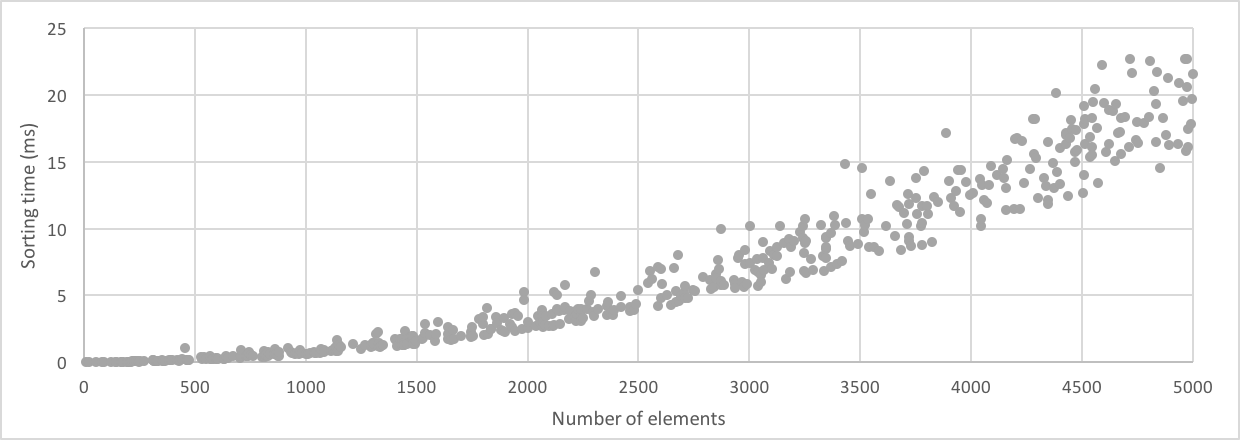
\includegraphics[width=130mm]{./img/sort_all_select.png}
		}
	}
	\centerline{
		\mbox{
			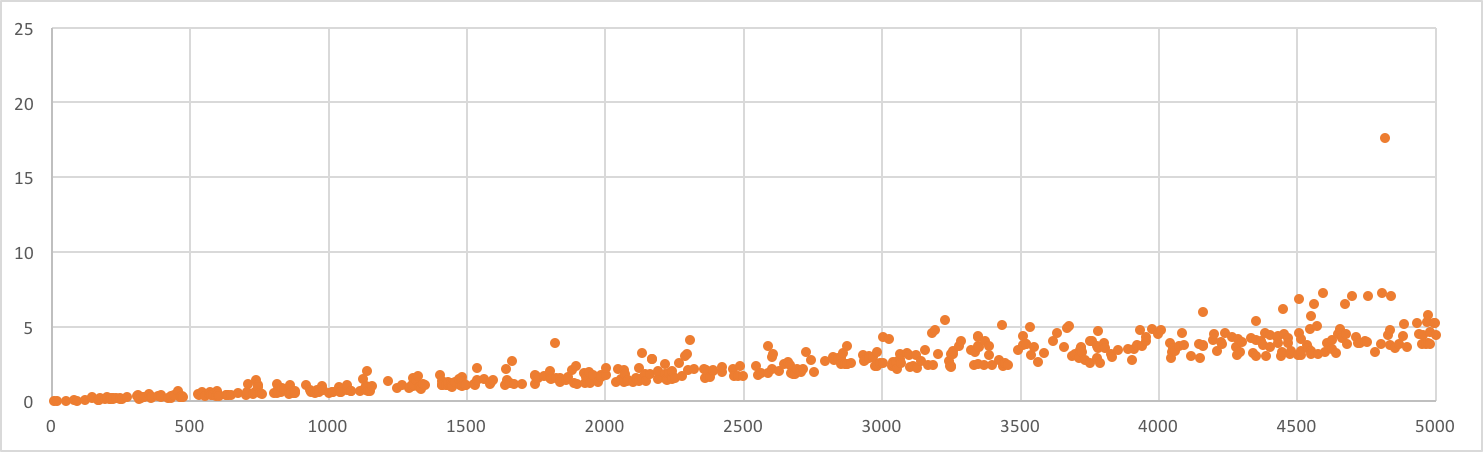
\includegraphics[width=130mm]{./img/sort_all_quick.png}
		}
	}
	\centerline{
		\mbox{
			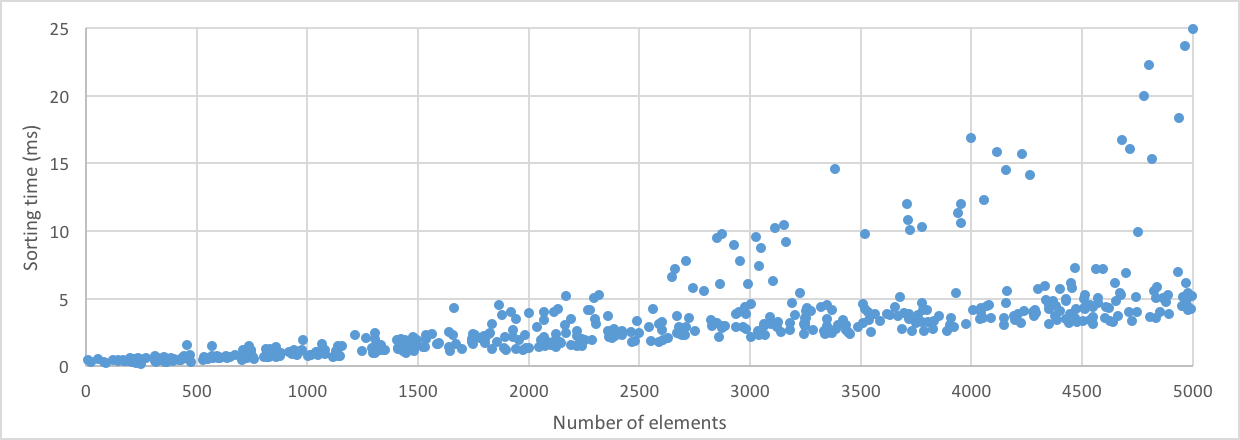
\includegraphics[width=130mm]{./img/sort_all_combined.png}
		}
	}
	\caption{Sorting times of sequences of different sizes using selection sort, quick sort and a combined function (from top to bottom).}
	\label{fig:sorting_graph_all}
\end{figure}

Figure \ref{fig:sorting_graph_all} shows us the execution times of quick sort, selection sort and the combined function (using the window-bound linear regression strategy) for different input sizes from this test. As we can see, the combined function times are mostly similar to the quick sort times. The figure \ref{fig:sorting_graph_start} shows only the interval between 0 and 1200, where selection sort tends to be better. The combined function has the worst performance, which is most likely caused by the selection overhead (see section \ref{subsec:strategy_perf}).


\begin{figure}[h!]
	\captionsetup{justification=centering,margin=0.5cm}
	\centerline{
		\mbox{
			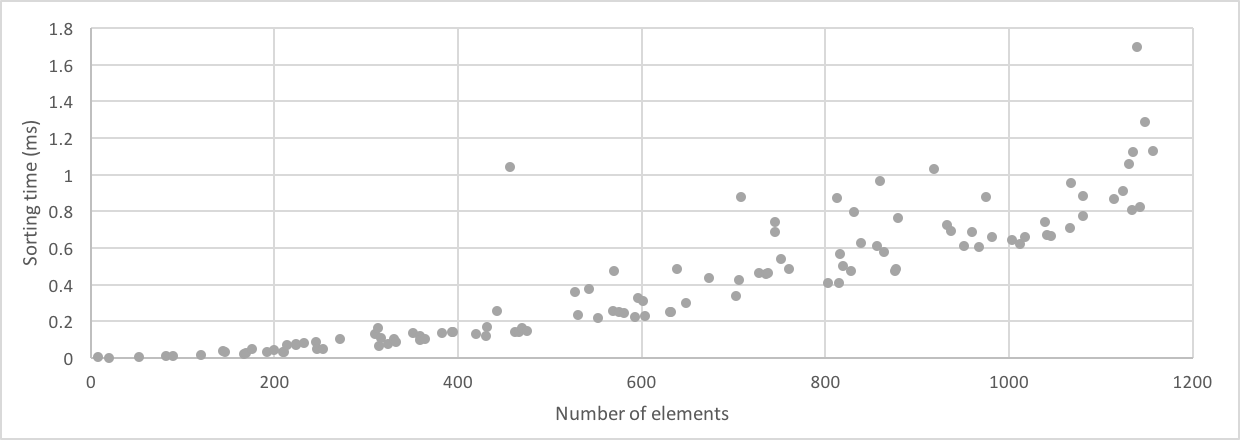
\includegraphics[width=130mm]{./img/sort_start_select.png}
		}
	}
	\centerline{
		\mbox{
			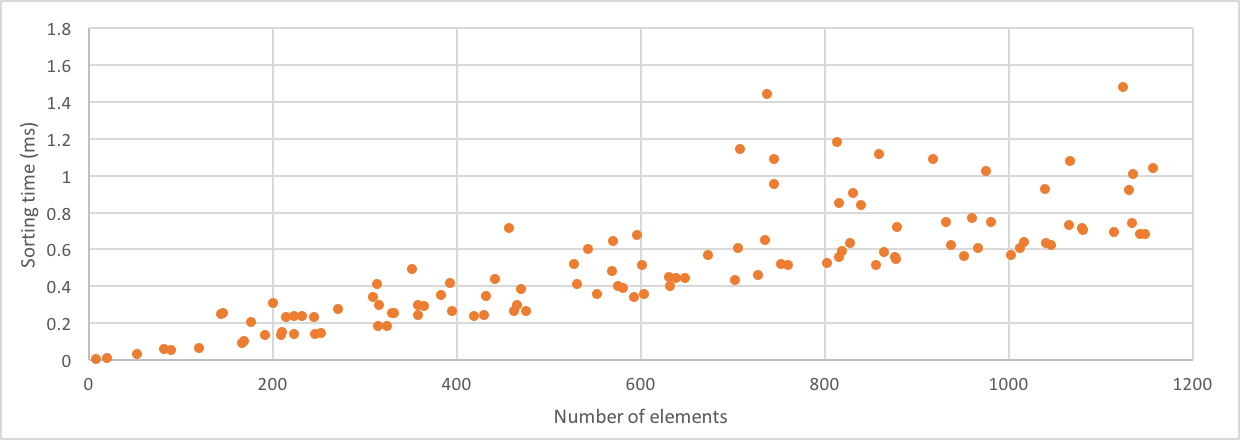
\includegraphics[width=130mm]{./img/sort_start_quick.png}
		}
	}
	\centerline{
		\mbox{
			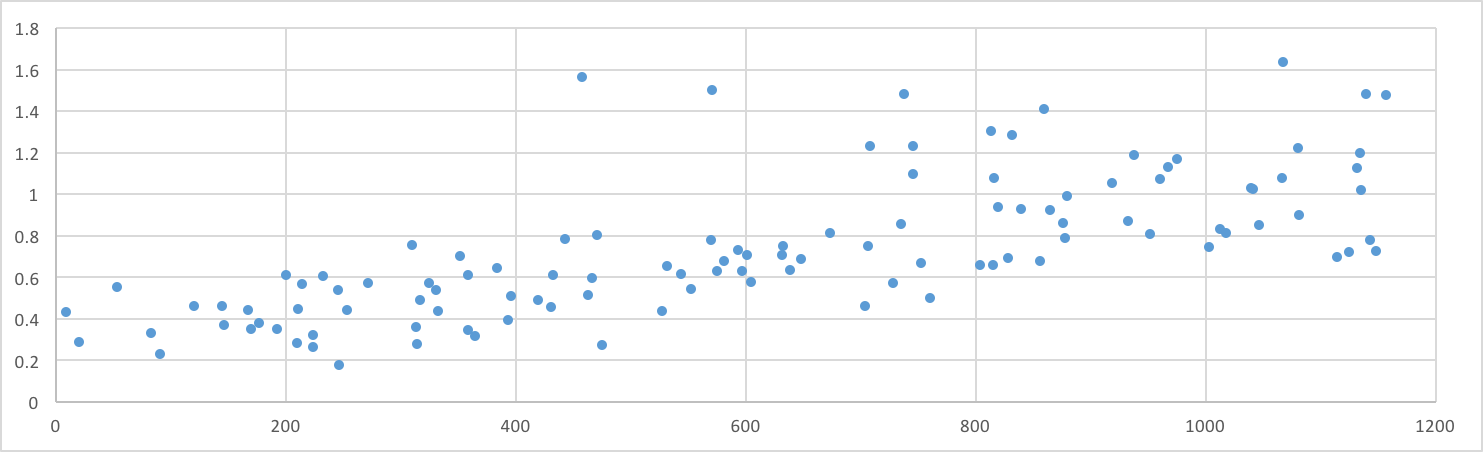
\includegraphics[width=130mm]{./img/sort_start_combined.png}
		}
	}
	\caption{Detailed view of the sorting times of sequences of different sizes using selection sort, quick sort and a combined function (from top to bottom).}
	\label{fig:sorting_graph_start}
\end{figure}

In conclusion, ScalaAdaptive is not suitable for performing optimization for very small inputs of various algorithms. The overhead time leads to worse performance overall, even though the selection is working fine and the better options are correctly selected.

\subsection{Matrix multiplication}

Another example of an algorithmic problem where ScalaAdaptive can be used is matrix multiplication. The basic multiplication algorithm has complexity of $O(N^3)$ and tends to get quite slow for larger matrices. A lot of more complex algorithms with slightly better complexities were discovered and are still being improved. The best achieved complexity so far is $O(N^{2.373})$ in \cite{williams_multiplying_2012}.

The practical problem with most of these fast algorithms is that they have high constants and therefore are not suitable for smaller matrices. In this test, we will use the ScalaAdaptive with the Strassen algorithm (complexity $O(N^{2.807})$, \cite{strassen_gaussian_1969}), and with the basic multiplication algorithm. We will use a simple implementation of both algorithms from \cite{noauthor_jlinalg_nodate}. The goal of this test is not to find the fastest way to multiply matrices, but to simply demonstrate that adaptation can be used with this class of algorithms to reach optimal results with almost no effort.

We tried generating 200 pairs of square matrices of random sizes between 50 and 900 filled with random integers. Then, we multiplied each pair using the basic algorithm, the Strassen algorithm, and the combined function. The window-bound linear regression strategy with $\alpha = 0.05$ was used. Because the run times are quite high in this case, the minimal number of observations before selection was lowered to 5 (using the \inlinecode{LowRunAwareSelectionStrategy}, see section \ref{subsubsec:selection_strategy_impl}). 

The results can be found in table \ref{tab:matrix_results}. As we can see, the overall results are in favor of the combined version. If we examine the relation between the run time and the size of the matrices in figure \ref{fig:matrix_mul_graph}, we can notice the unusual character of the Strassen algorithm which is caused by it rounding up the matrix to the size corresponding to a closest power of two. This kind of an input dependency does not work well with linear regression, especially around the edges, and should optimally be used with logarithmic grouping and a mean based strategy. Nevertheless, the selection process worked fine enough and chose the optimal algorithm for almost all the inputs.

\begin{table}[]
	\captionsetup{justification=centering,margin=0.5cm}
\bgroup
\def\arraystretch{1.5}%
\begin{center}
	\begin{tabular}{|l|r|}
		\hline
		& \multicolumn{1}{l|}{\textbf{Total time (s)}} \\ \hline
		\textbf{Basic algorithm}    & 2230.21                                      \\ \hline
		\textbf{Strassen algorithm} & 2168.29                                       \\ \hline
		\textbf{Combined (LR)}      & 1673.63                                       \\ \hline
	\end{tabular}
\end{center}
\egroup
\caption{Total times of multiplying 200 pairs of square matrices of sizes 50-900.}
\label{tab:matrix_results}
\end{table}


\begin{figure}[h!]
	\captionsetup{justification=centering,margin=0.5cm}
	\centerline{
		\mbox{
			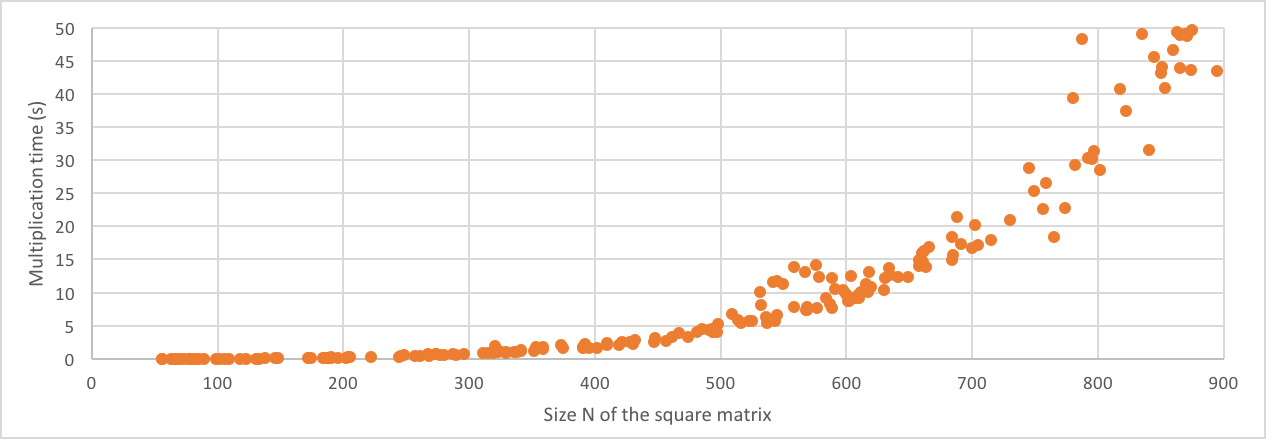
\includegraphics[width=130mm]{./img/matrix_mul_basic.png}
		}
	}
	\centerline{
	\mbox{
		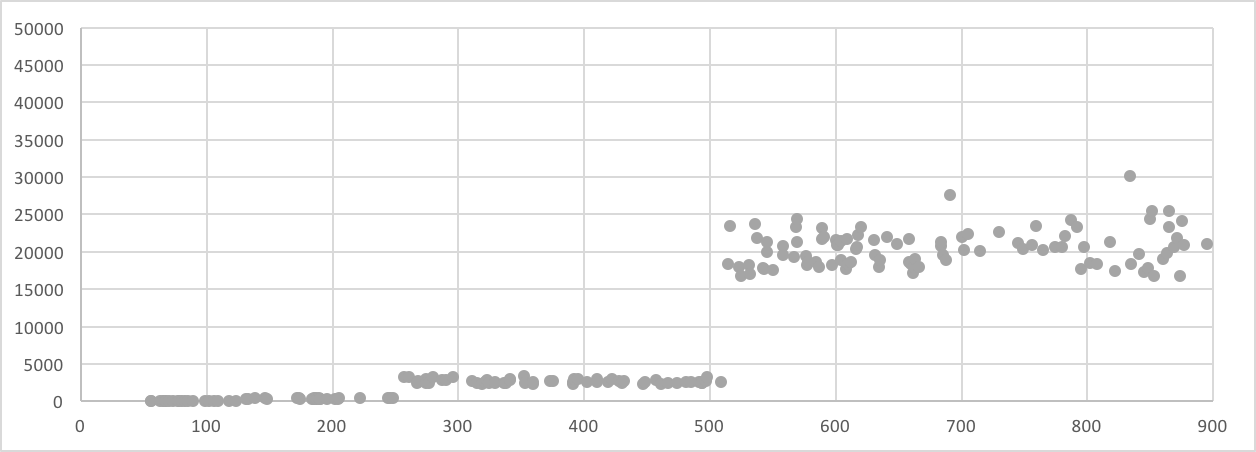
\includegraphics[width=130mm]{./img/matrix_mul_strassen.png}
	}
}
	\centerline{
	\mbox{
		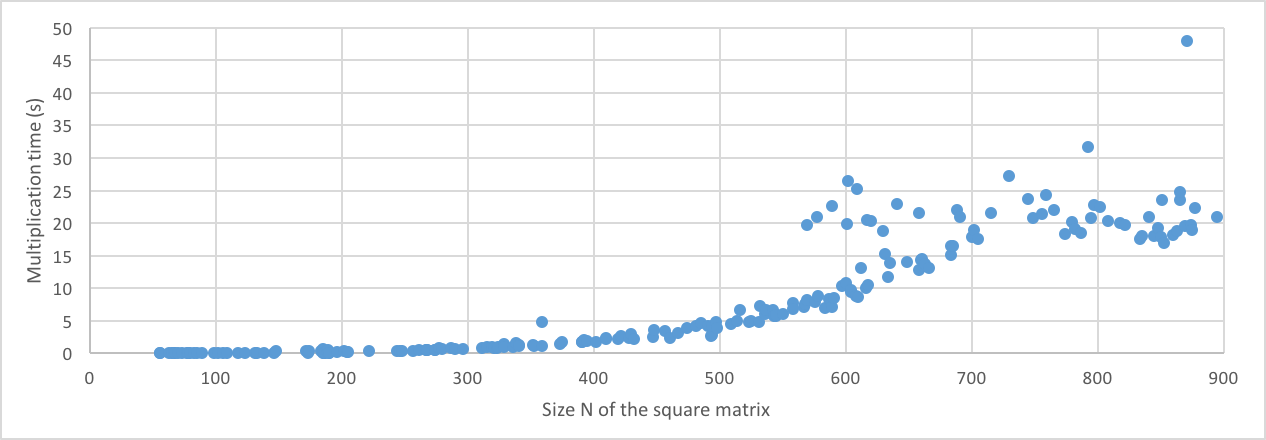
\includegraphics[width=130mm]{./img/matrix_mul_combined.png}
	}
}
	\caption{Multiplication times of matrices of different sizes using basic algorithm, Strassen algorithm and a combined function (from the top to the bottom).}
	\label{fig:matrix_mul_graph}
\end{figure}

The matrix multiplication algorithms represent an ideal problem for the adaptive execution. Current approach to designing a fast library method for multiplying matrices would consist of measuring the matrix size limit where the more complex algorithm becomes faster than the basic one and then putting a branching on a fixed size test in the method, deciding which one to use. With ScalaAdaptive framework, this whole process can be skipped, and if the algorithms change, the system will adapt, finding the new limit by itself.

\subsection{JSON parsing}
\label{subsec:json_parsing}

JSON\footnote{JavaScript Object Notation} is a data-exchange format that can hold serialized object trees and collections. It is based on the notation for object (technically key-value dictionaries) literals in JavaScript. The format has recently become extremely popular due to its simplicity, data efficiency and readability, and as of today, is basically a standard for HTTP REST APIs. Most of the systems with distributed architecture that communicate over such an API (typically client-server applications) need to serialize and deserialize JSON upon sending a request or receiving a response, which might occur quite often.

The problem concerning JSON and other similar formats (XML, ProtocolBuffers, etc.) is that there is a variety of libraries available to perform the serialization and deserialization, and we have to decide for one when designing our application. The API tends to be similar and since it is used with such a frequency, optimizing its performance might be a suitable goal. There are performance tests and comparisons of the libraries available, but as shown in \cite{dreyfuss_ultimate_2015}, each one might be suitable for a different use case. In addition, \cite{Trojanek:Thesis:2013} shows that the performance might significantly vary in different versions.

This library decision problem is a suitable use-case for ScalaAdaptive -- we can create a simple wrapper library with the same API as the original libraries that will expose the functions combined from the original serialization and deserialization methods. The user will be abstracted from the ScalaAdaptive, and the libraries can be added or removed at any time very easily.

\subsubsection{Combining GSON and Jackson}

In \cite{dreyfuss_ultimate_2015} we can find a benchmarks of the most popular JSON libraries from the Java world. For the test, we chose to use GSON\footnote{Version 2.8.1 of the GSON library from Maven repository was used in the test.} and Jackson\footnote{Version 2.8.8 of the Jackson library from Maven repository was used in the test.}. We will measure only the deserialization part (parsing of string containing JSON), which is the more time-complex operation. 

The combined function was created in the following way:
\lstset{style=Scala}
\begin{lstlisting}
val parse = (
  parseWithGson _ or parseWithJackson
  groupBy ((json, c) => GroupId(Math.log(json.length).toInt))
  selectUsing Selection.MeanBased
  withPolicy new PauseSelectionAfterStreakPolicy(10, 200)
)
\end{lstlisting}

The test is based on parsing three different JSON strings:

\begin{itemize}
	\item Small - 9KB, 10 records array
	\item Medium - 80KB, 100 records array
	\item Large - 8MB, 1000 records array
\end{itemize}

We know that we deal with fixed sizes of input files, so we can use the default t-test selection strategy without any problems, because every size will occupy one of the groups. If we knew that the sizes within a group might vary, we should use some other strategy. The value $\alpha = 0.05$ is used.

\begin{table}[h!]
	\captionsetup{justification=centering,margin=0.5cm}
	\bgroup
	\def\arraystretch{1.5}%
	\begin{center}
		\begin{tabular}{ | l | r | r | r | }
			\hline
			& \textbf{GSON} & \textbf{Jackson} & \textbf{Combined} \\ \hline
			10000 * Small JSON & 1830.36 & 4883.24 & 2566.54 \\ \hline	
			Small JSON average & 0.18 & 0.49 & 0.26 \\ \hline	
			5000 * Medium JSON & 4865.89 & 3142.05 & 3059.18 \\ \hline	
			Medium JSON average & 0.97 & 0.63 & 0.61 \\ \hline	
			200 * Large JSON & 15790.47 & 7298.75 & 7740.31 \\ \hline	
			Large JSON average & 78.95 & 36.49 & 38.70 \\ \hline
			\textbf{Total time} & 22486.71 & 15324.05 & 13366.03 \\
			\hline
		\end{tabular}
	\end{center}
	\egroup
	\caption{Results of the JSON parsing tests (times in ms).}
	\label{tab:json_parsing_results}
\end{table}


During the test, we ran each one of the three parsing functions 10000 times on the small JSON, 5000 times on the medium JSON and 200 times on the large JSON. We added up run times on these inputs for all the functions, and the results can be seen in the table \ref{tab:json_parsing_results}.

\begin{table}[h!]
	\captionsetup{justification=centering,margin=0.5cm}
	\bgroup
	\def\arraystretch{1.5}%
	\begin{center}
		\begin{tabular}{ | l | r | r | r | }
			\hline
			& \textbf{GSON} & \textbf{Jackson} & \textbf{Combined} \\ \hline
			10000 * Small JSON  & 2180.20       & 5615.20          & 5667.64           \\ \hline
			Small JSON average  & 0.22          & 0.56             & 0.57              \\ \hline
			5000 * Medium JSON  & 4696.52       & 2944.04          & 3889.25           \\ \hline
			Medium JSON average & 0.94          & 0.59             & 0.78              \\ \hline
			200 * Large JSON    & 15829.39      & 7433.50          & 7772.41           \\ \hline
			Large JSON average  & 79.15         & 37.17            & 38.86             \\ \hline
			\textbf{Total time}          & 22706.11      & 15992.73         & 17329.30          \\ \hline
		\end{tabular}
	\end{center}
	\egroup
	\caption{Results of the JSON parsing tests without the policy applied (times in ms).}
	\label{tab:json_parsing_results_no_policy}
\end{table}

As we can see, the combined function time is a little worse that the better alternative for each input size separately. But since the better alternative changes for different inputs, the total time of the combined function is the best.

We can compare the results with table \ref{tab:json_parsing_results_no_policy} showing the same test, only without the \textbf{Pause selection after streak} policy. We see that by actually performing the selection every time, the overhead grows, which is noticeable especially on the small and medium inputs, where the results are significantly worse. Applying the overhead-limiting policies therefore makes sense and can cause significant performance differences.

\subsection{Load balancing}

A different sort of problems that ScalaAdaptive might help with concerns adapting systems to environment changes. We can demonstrate this on a simple example -- an application that relies on a remote web service running in multiple instances on different web servers. The service itself is stateless, so the requests can be performed on any of them.

The main goal of such a replication is usually to distribute the work between more nodes, so that the response times remain low. A technique called load balancing should take care of distributing the requests evenly between the nodes often just using a simple round-robin technique. This, however, has to be done on the side of the service, through a common gateway. 

We will use ScalaAdaptive to implement a simple load balancing on the side of the client by evaluating the response times and selecting the target node using our selection strategies. We will take advantage of the possibility to limit the maximal age of the historical data (see section \ref{subsec:limiting_record_age}) - we want to make decisions based only on the most recent measurements, because we suppose that they will change rapidly.

There are two goals of this load balancing example:

\begin{itemize}
	\item To provide better performance than relying just on one node
	\item To limit the load on the node that is currently under pressure (and thus slow)
\end{itemize}

Suppose we have a simple web service running on multiple nodes and a system that performs synchronously running requests to these nodes. The request has the following form:

\lstset{style=Scala}
\begin{lstlisting}
def request(url: String)(query: String): Option[String] = ???
\end{lstlisting}

We can take advantage of the possibility to curry the function and create the composed request that works with multiple nodes using the ScalaAdaptive API in the following way:

\lstset{style=Scala}
\begin{lstlisting}
private def getRequest(s: Server) = 
  IdentifiedFunction(performRequest(s.url) _, s"request_${s.name}")
val balancedRequest =
(
  servers.tail.foldLeft(getRequest(servers.head)) { (f, s) =>
    f.or(getRequest(s)) }
  selectUsing Selection.MeanBased
  limitedTo Duration.ofSeconds(20)
)
\end{lstlisting}

Note that we need to use the custom identifier feature as mentioned in \ref{subsubsec:custom_identifier}, because the function is combined from a single eta-expanded method with different arguments fixed in the currying process. The closure type is therefore the same for all the resulting functions. The selection will be done using the default t-test strategy with $\alpha = 0.05$.

For the actual test, we used two instances of a simple custom web service running on different ports of the same machine. Its implementation can be found in attachment \ref{attach:cd}. We simulated the problems with load on the machines by artificially changing the response times of the servers every 50 seconds according to a set of predefined scenarios. From the client application, we sent one request every 0.5 seconds directly to each one of the servers and one using our balanced method. 

The results for three different scenarios can be seen in figure \ref{fig:load_balance_scen}. The lines represent response time evolution in time - direct requests are marked with double line and dotted line, the balanced request is solid. We can observe that most of the time, the solid line copies the lower of the two remaining lines. Sometimes, it repeatedly reaches the higher line, which means that the balanced request is sent to the slower server in order to gather fresh run data.

\begin{figure}[h!]
	\captionsetup{justification=centering,margin=0.5cm}
	\centerline{
		\mbox{
			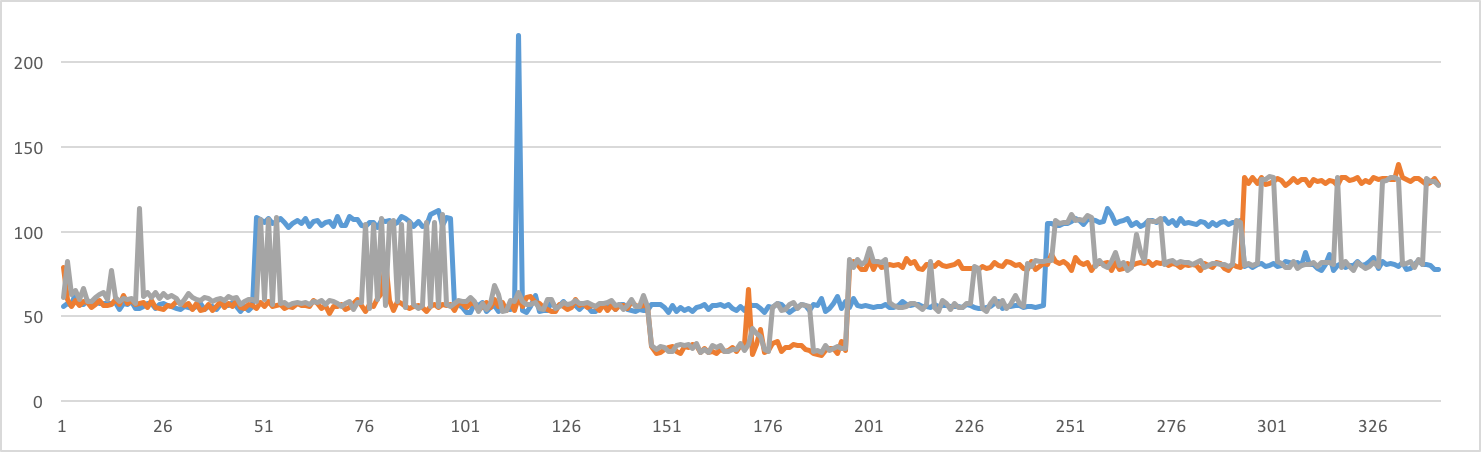
\includegraphics[width=130mm]{./img/load_balance_scen1.png}
		}
	}
	\centerline{
		\mbox{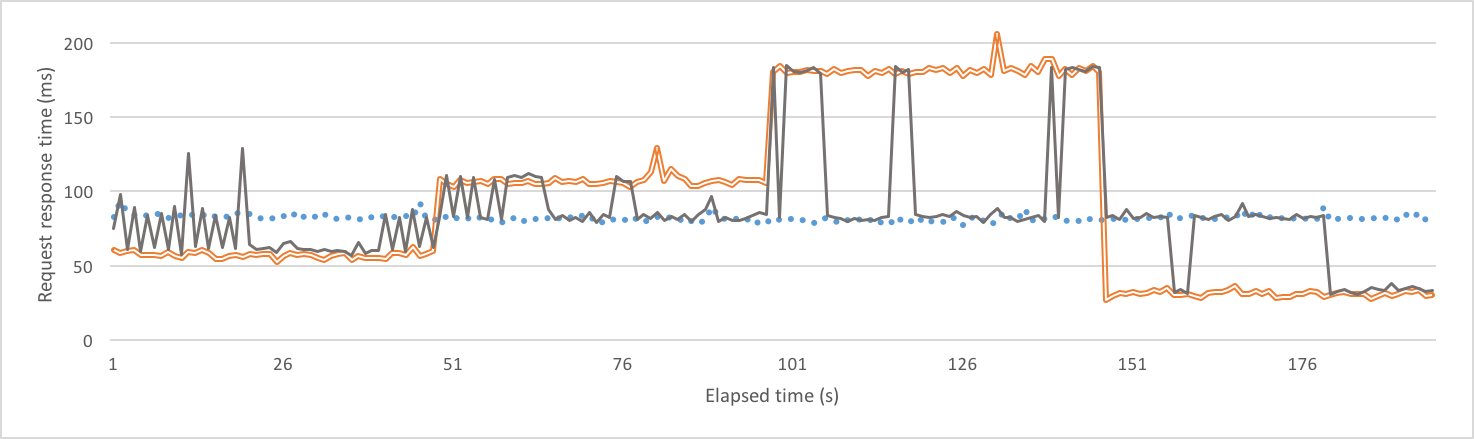
\includegraphics[width=130mm]{./img/load_balance_scen2.png}}
	}
	\centerline{
		\mbox{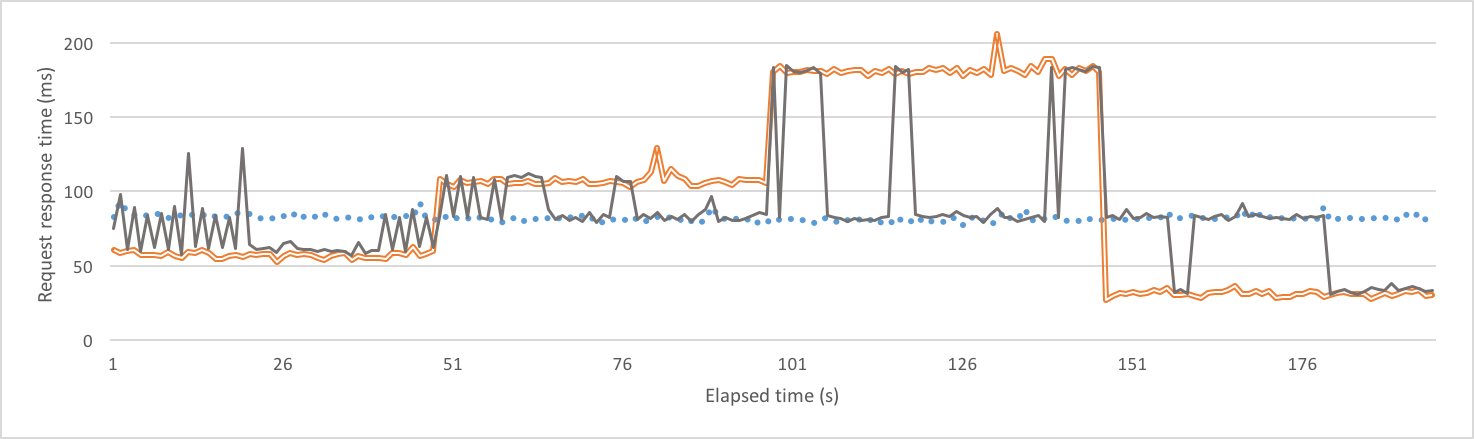
\includegraphics[width=130mm]{./img/load_balance_scen3.png}}
	}
	\caption{Time evolution of response times for request methods in scenarios 1, 2 and 3 (from top to bottom).}
	\label{fig:load_balance_scen}
\end{figure}

The average response times in these scenarios are shown in the table \ref{tab:load_balance_resp_avgs}. The balanced response time is always lower than the worse of the response times. In case where the load alternates between the two servers (scenario 2), the balanced version has the best average response time. If, on the other hand, only one server fluctuates and the other one keeps a relatively low response time (scenario 3), the balanced version is slightly worse than the optimal one. Nevertheless, the second goal of moving the load between the servers is completed in all three scenarios.

\begin{table}[h!]
	\centering
	\captionsetup{justification=centering,margin=0.5cm}
		\bgroup
	\def\arraystretch{1.5}%
	
	\begin{tabular}{|l|r|r|r|}
		\hline
		& \textbf{Server 1}& \textbf{Server 2}& \textbf{Balanced}\\ \hline
		Scenario 1 & 74.20             & 70.48             & 68.38             \\ \hline
		Scenario 2 & 80.92             & 81.77             & 72.52             \\ \hline
		Scenario 3 & 81.97             & 94.39             & 85.38             \\ \hline
	\end{tabular}
	\egroup
	\caption{Average response times for the request methods in scenarios 1, 2 and 3 (in ms).}
\label{tab:load_balance_resp_avgs}
\end{table}

A disadvantage of ScalaAdaptive that complicates the usage in this area is the fact that it does not support measuring run times of asynchronous functions, i.e. functions that perform callbacks or complete promises upon finishing.

\section{Apache Spark}

Apache Spark (\cite{noauthor_apache_nodate}) is a framework for distributed computing that is focused on data processing in a similar way as the MapReduce distributed computation paradigm. It works with distributed data sets that can be mapped, filtered, grouped or reduced, but unlike the implementations in Hadoop or other systems, it is focused on in-memory data processing on the nodes. Currently, it is one of the most used systems in big data processing, designed to work with a large variety of distributed storage systems (e.g. HDFS, Cassandra, OpenStack Swift).

The Spark framework represents one of the most interesting possibilities to use the ScalaAdaptive framework. The data processing queries are long-running tasks, so any overhead imposed by the selection is negligible. On the other hand, the potentially saved time on a faster implementation increases. In addition, the distributed computation model and the necessity to create an execution plan which depends on the data locations, sizes, etc. leads to large differences in execution times based on:

\begin{itemize}
	\item The query itself
	\item The cluster it is running on (number of machines, cores, network)
	\item The configuration of Apache Spark
\end{itemize}

The goal of this section is to show the basic ideas where the adaptivity might be used in such a framework.

\subsection{Spark APIs}
\label{subsec:spark_apis}

Spark currently supports three different APIs that can be used to construct Spark queries.

\subsubsection{RDD}

RDD (Resilient Distributed Dataset) was the first API introduced and is basically a distributed dataset of JVM objects. Spark is not aware of the structure of the internal JVM objects, it is treating the individuals like blackboxes. The RDD query is typed and constructed using lambda expressions that work with these objects:

\lstset{style=Scala}
\begin{lstlisting}
rdd.filter(_.id > 5000).count
\end{lstlisting}

Upon execution, the Spark worker engine manipulates with the RDDs as a whole (partitions it, collects the results, etc.), but the operations on its members (filtering, transformation, grouping) are carried out by actually executing the lambda functions.

This approach is very simple and allows the user to write queries over custom data types without any limitation. The downside is that the Spark execution engine does not know what is going on within the lambdas, cannot optimize the execution plan based on the query, and, when moving the parts of RDDs between the nodes, the objects have to be serialized and deserialized again.

\subsubsection{DataFrames and Spark SQL}

DataFrames API was introduced later into the Spark framework with a goal of solving the problems of RDDs. The data within DataFrames are described by a schema, somehow similar to classic SQL schema - Spark knows exactly how are the data records structured. The queries are constructed using Spark SQL, a query language (DSL in Scala) that uses textual names of the record attributes (i.e. schema columns). As we can see in the following example, the actions are described by strings and parsed by Spark upon execution:

\lstset{style=Scala}
\begin{lstlisting}
df.filter("id > 5000").count
\end{lstlisting}

Spark therefore knows how exactly the mapping, filtering, reducing or grouping is going to happen, and can use these information to optimize the execution and data distribution, to make estimations, etc., when building the query plan. In addition, the data described by a schema can be easily persisted or transfered between nodes without the need to perform a JVM serialization. A major disadvantage is the necessity to provide the schema and the fact that the actual query is parsed at runtime and is untyped - errors in attribute names or conditions in general will not be detected upon compilation.

\subsubsection{Datasets}

The newest Spark API, Datasets, was designed with an objective of combining the best from RDD and DataFrame approaches. The query programming API is typed and works with JVM objects, just like RDD, but the internal representation is schema-based, like in DataFrames. In order for this to work, Spark uses a mechanism of encoders that can transform the JVM representation to the internal one and vice-versa. It also analyzes the content of the typed lambdas and uses the same optimization as with the DataFrames API.

\subsection{ScalaAdaptive tests}

To perform the test of ScalaAdaptive with Apache Spark, two environments were used:

\begin{itemize}
	\item Spark local mode with 1 worker\footnote{Using \inlinecode{master("local[1]")} setup.} on a laptop with quad-core 1.3 GHz Intel Core i5 processor and 8GB of RAM
	\item Spark local mode with 8 workers\footnote{Using \inlinecode{master("local[8]")} setup.} on the same machine
	\item Cluster of 12 Spark workers deployed in Docker containers on 3 machines, each with two 8-core Intel Xeon CPU E5-2660 0 @ 2.20GHz and 48GB of RAM
\end{itemize}

Randomly generated data were used for the test, no distributed storage was involved. The tests were running with the \inlinecode{StorageLevel.MEMORY\_ONLY} data persistence configuration. The version 2.1.0 of the Apache Spark library was used.

\subsubsection{Query selection}

The most simple adaptation case that can be applied to any data processing or querying framework is the query selection. A data operation can usually be expressed using a variety of queries that differ in the order or character of the elementary steps. These queries can have different performance, based on the optimizations that the executing engine can perform, especially in the distributed environment where the main concern is keeping the amount of data transfered to the minimum.

An example of such a query performance variation can be the \textit{group} versus \textit{reduce} problem. Suppose have a set of key-value pairs and we want to group them by key and then reduce the groups (by aggregating their content somehow). The straightforward approach is to group the data and to map the aggregation function over the grouped values:

\lstset{style=Scala}
\begin{lstlisting}
data.groupByKey()
      .map(i => (i._1, i._2.flatten.toArray))
\end{lstlisting}

Because the execution engine does not understand the mapping action (RDDs do not analyze the queries), this requires the grouping to be done across all the workers to physically create the groups, even though we are just going to immediately reduce them. 

To address this issue, a special operation for reducing is present in the API:

\lstset{style=Scala}
\begin{lstlisting}
data.reduceByKey((arr1, arr2) => arr1 ++ arr2)
\end{lstlisting}

In this case, the reduced value can be first computed for each node out of the records with given key present on the node. Then, the partial reduction results can be passed around and further aggregated.

A test with ScalaAdaptive was performed on a 5000 key-value pair sequence in Local[8] mode. The two RDD queries presented in this section were combined together and the resulting function was executed 1000 times. The framework decided correctly for the reduce variant using the default t-test with $\alpha = 0.05$. The analytics data show the following average run times of the queries:
\begin{itemize}
	\item \textbf{GroupByKey} -- 3677.61ms
	\item \textbf{ReduceByKey} -- 684.52ms
\end{itemize}

\subsubsection{RDDs or Datasets}

As explained in section \ref{subsec:spark_apis}, Spark has various APIs that allow the user to perform the query. Theoretically, the Dataset API should offer the same expressiveness and better performance. A lot of current production Spark code is, however, written in RDDs, as it was the first (and the only for some time) presented API. This poses a question whether the code should be kept and maintained in RDDs, or whether it would be better to replace it with Datasets and what the eventual performance gain would be.

The ScalaAdaptive can be used in this case to limit the potential negative impact of this change. The Dataset-based queries can be implemented into the system and wrapped along with the old RDD queries into a single combined query. If there was a place where the Dataset query would, for some reason, have worse performance, the ScalaAdaptive framework should discover it and keep using the old RDD query. In the longer term, the results of ScalaAdaptive selections can be evaluated and used to discover problematic queries and to decide about next steps.

In this test, we are going to try combining two queries from the two different APIs and try them out in different environments and with different data sizes. We are going to track the execution times of both of them in the phase where the data is gathered in a round-robin manner, and then analyze the decision made by the ScalaAdaptive framework. We would preferably like to find out whether the decision will be the same for all the data and environments, or whether there are going to be significant differences.

For the test, we implemented the following two queries in both RDDs and Datasets:
\begin{itemize}
	\item \textbf{Query 1} -- generates $n$ random key-value pairs using parallelized RDD generation, groups by the key and counts the groups
	\item \textbf{Query 2} -- generates $n$ records with multiple attributes from in-memory sequence, filters them by an attribute, groups them by a different attribute, reduces the groups into new records, filters the records again and groups them for the second time
\end{itemize}

The RDD and Dataset option of each of the queries were combined together and the result was executed $100$ times in various environments and with multiple values of $n$. The average execution times of the queries, as retrieved from the analytics data (see section \ref{subsubsec:analytics}), can be seen for all the cases in table \ref{tab:spark_adaptive_rdd_vs_ds_test}. The last column shows the ScalaAdaptive decision after gathering enough data -- default t-test selection strategy with $\alpha = 0.05$ was used.

We can see that it is definitely not possible to assume that Datasets are generally faster than RDDs. The only situation where Dataset got better performance was the Query 1 test with the largest amount of data. We can observe that at least for Query 1, the Datasets perform better for larger data sizes, both locally and in the cluster. For Query 2, it seems that Dataset performance is constantly around 7 times worse than the RDD performance.

These observations might be caused by Datasets having the operations optimized to different cases, or even by our wrong selection of Dataset alternatives of the RDD queries. But such a case might be a real scenario where the ScalaAdaptive framework can be successfully employed and help to discover a potential problem.

\begin{table}[h!]
	\centering
	\captionsetup{justification=centering,margin=0.5cm}
	\bgroup
	\def\arraystretch{1.5}%
	\begin{tabular}{|l|r|r|r|}
		\hline
		& \multicolumn{1}{c|}{\textbf{RDD}} & \multicolumn{1}{c|}{\textbf{Dataset}} & \multicolumn{1}{c|}{\textbf{ScalaAdaptive decision}} \\ \hline
		Query 1: Cluster 500000       & 920.97                            & 1633.84                           & RDD                                                  \\ \hline
		Query 1: Cluster 2000000      & 7105.58                           & 7068.34                           & Cannot decide                                         \\ \hline
		Query 1: Cluster 5000000      & 37140.28                          & 3587.97                           & Dataset                                                  \\ \hline
		Query 1: Local{[}1{]} 200000  & 2426.95                           & 12554.66                          & RDD                                                  \\ \hline
		Query 1: Local{[}8{]} 200000  & 1499.14                           & 7446.45                           & RDD                                                  \\ \hline
		Query 1: Local{[}8{]} 1000000 & 12070.14                          & 12861.32                          & Cannot decide                                         \\ \hline
		Query 2: Cluster 100000 & 1152.19 &	6956.03 & RDD \\ \hline
		Query 2: Cluster 1000000      & 2162.72                           & 14311.13                          & RDD                                                  \\ \hline
	\end{tabular}
\egroup
\caption{Run times (in ms) of Spark queries on RDD and Datasets in various environments.}
\label{tab:spark_adaptive_rdd_vs_ds_test}
\end{table}

\subsubsection{Spark SQL adaptive execution}

Spark queries are divided into stages, where each stage can be performed on a single node without the need to exchange any data. Typically, multiple maps or filters are chained within one stage, because every record can be mapped without the necessity of any other data. On the other hand, join, group and reduce operations have to be done at the beginning of a new stage, because they can potentially require data from other nodes. Before every stage, a shuffle is performed - the data is exchanged between the nodes. 

The data is divided into partitions and each node processes a specific subset during the stage execution. Upon shuffle, some partitions get exchanged. Originally, the partitioning of the data following each shuffle was fixed and based on the original partitioning - it did not reflect the actual results of previous stages, which could potentially lead  to some nodes having a lot less work than the others if there were partitions with majority of data filtered out in previous stage. To solve this issue, an experimental feature called \textit{adaptive execution}\footnote{Should not be mistaken with the adaptive execution of \textit{ScalaAdaptive} framework.} was introduced into Spark SQL. It causes that the result sizes from previous stages are collected and a new partitioning is created before performing the shuffle.

The \textit{Spark adaptive execution} feature is turned off by default. We can use ScalaAdaptive to experiment with the performance impact when enabling it. In addition, there are two configurable attributes of the feature:
\begin{itemize}
	\item \inlinecode{targetPostShuffleInputSize} - the optimal size of a partition (will be targeted during shuffle)
	\item \inlinecode{minNumPostShufflePartitions} - the minimal number of partitions (will be strictly kept)
\end{itemize}
We can try a custom value for these attributes in one of the ScalaAdaptive combinations.

The usage of ScalaAdaptive in this case will, however, be a little more complicated. Some attributes of the Spark SQL configuration can be changed at any point in the execution, but doing so is not reliable, especially in large cluster - changes do not seem to be reflected immediately. A safer approach is to create the SparkSession already with the target configuration. If we create new session for each query, we can incorporate the session creation into the query function. If we, on the other hand, use one session for multiple queries, we need to split the selection process (session creation) and the measurement process (query execution). The only solution is the delayed measurement model described in section \ref{subsec:delayed_measuring}.

The test was performed on a Dataset of $n$ records which was filtered, grouped by an attribute, the groups reduced to a single element and the result filtered again and counted. We tried to combine various values of $n$ with the following setups:

\begin{enumerate}
	\item \textit{Spark adaptive execution} disabled (currently the default configuration)
	\item \textit{Spark adaptive execution} enabled with default attributes
	\item \textit{Spark adaptive execution} enabled\\
	\inlinecode{targetPostShuffleInputSize} = 512MB\\
	\inlinecode{minNumPostShufflePartitions} = -1 (unlimited)
	\item \textit{Spark adaptive execution} enabled\\
	\inlinecode{targetPostShuffleInputSize} = 2MB\\
	\inlinecode{minNumPostShufflePartitions} = 200
\end{enumerate}

The SparkSession was created 12 times for every test case and the query was executed 10 times using each session (120 executions in total). As the \inlinecode{LowRunAwareSelectionStrategy} (see section \ref{subsubsec:selection_strategy_impl}) was set to a minimum of 20 records, each of the setups had to be used to create at least two sessions. The t-test selection strategy with $\alpha = 0.05$ was used.


\begin{table}[h!]
	\centering
	\captionsetup{justification=centering,margin=0.5cm}
	\bgroup
	\def\arraystretch{1.5}%
	\begin{tabular}{|l|r|r|r|r|r|}
		\hline
		& \multicolumn{1}{c|}{\textbf{1.}} & \multicolumn{1}{c|}{\textbf{2.}} & \multicolumn{1}{c|}{\textbf{3.}} & \multicolumn{1}{c|}{\textbf{4.}} & \multicolumn{1}{c|}{\textbf{\begin{tabular}[c]{@{}c@{}}ScalaAdaptive\\ decision\end{tabular}}} \\ \hline
		Local{[}8{]} 1000  & 4322.24                          & 1472.51                          & 1916.87                          & 3528.62                          & Cannot decide                                                                                  \\ \hline
		Local{[}8{]} 10000 & 6911.03                          & 4499.11                          & 4933.53                          & 6320.43                          & Cannot decide                                                                                  \\ \hline
		Cluster 20000      & 1234.36                          & 725.79                           & 3892.56                          & 1172.69                          & 2.                                                                     \\ \hline
		Cluster 200000     & 2879.25                          & 2538.94                          & 5639.02                          & 2853.10                          & 2.                                                                             \\ \hline
	\end{tabular}
	\egroup
	\caption{Average run times (in ms) of Spark queries with different configurations in various environments, and the configurations that ScalaAdaptive selected.}
	\label{tab:spark_adaptive_config_test}
\end{table}

The table \ref{tab:spark_adaptive_config_test} shows the average execution times for the setups based on the initial 20 runs. It additionally marks if the framework reached a decision after having evaluated these runs. As we can see, the performances of the options vary a lot depending on the input size and on the execution environment. The default configuration (with \textit{Spark adaptive execution} disabled) in the local execution on small data is by far the worst, in large cluster is among the better ones. The configuration number 2, i.e., the manually activated \textit{adaptive execution} with default setup, is the best in all the cases, but we can see that the results tend to change a lot. Using ScalaAdaptive can therefore help discover eventual better configurations.

The disadvantage of ScalaAdaptive in this case is that selection from quite a lot of alternatives is required, which suffers from multiple problems discussed in chapter \ref{chap:deciding}. In case of the results discussed, the test was not able to decide in the two local setups, which lead to looping through all the options including the worst ones.

\section{Problems with the practical use of the framework}

Using adaptive framework in the development process is a new concept with many consequences. While designing, implementing and evaluating the framework, we discovered a few potential problems that can complicate its practical application.

\subsection{Invocation overhead}

The framework adds a non-trivial overhead to the function invocation process due to the selection and the storing of the evaluation data. In order to limit this, the policy-based invocation system was added to the framework with a goal of skipping the selection in some situations. Therefore, two different types of overhead time per invocation can be measured:

\begin{enumerate}
	\item \textbf{Policy evaluation overhead}\\
	Part of every invocation. It is expected to be small and it should be constant throughout the whole application lifetime. It cannot be measured from within the framework, but it can be computed by measuring the combined function run time and then by subtracting the run time and overhead time from the \inlinecode{AnalyticsData} collected by the function.
	\item \textbf{Selection overhead}\\
	Exists only when the SelectNew or GatherData result is given by the policy. It is determined by the actual selection strategy used and is in general expected to be longer and to be related to the amount of historical data available for the functions involved. It is tracked by the framework and included in the \inlinecode{AnalyticsData} and in addition, it is one of the statistics that the policies are based on.
\end{enumerate}

The figure \ref{fig:overhead_sel_policy} shows these times tracked for a sequence of 20000 invocations (sampled every 50th run) of a sample combined function using the window-bound linear regression strategy (see section \ref{subsec:window_bound_regression}) and a policy that emits the SelectNew result every time. We can see that the selection overhead is significantly larger and really grows with the number of records. The policy evaluation overhead remains basically constant.

\begin{figure}[h!]
	\captionsetup{justification=centering,margin=0.5cm}
	\centerline{\mbox{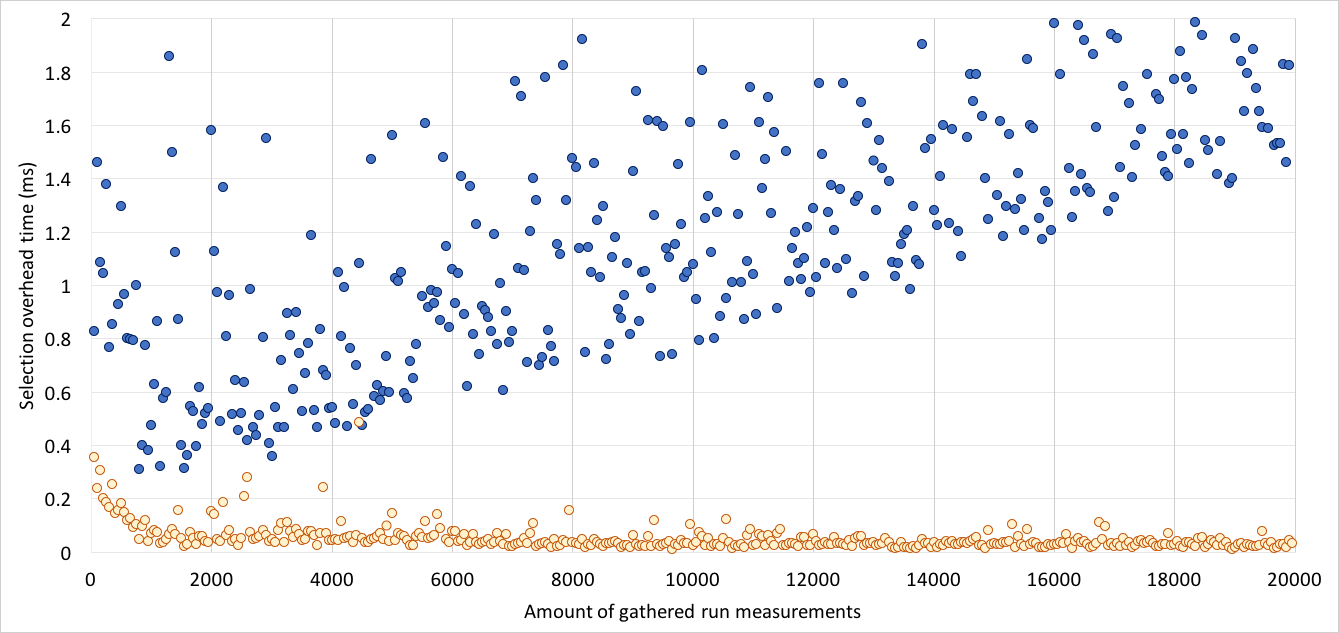
\includegraphics[width=140mm]{./img/overhead_sel_policy.png}}}
	\caption{Selection overhead times (dark) and policy evaluation overhead times (light), both in ns, for a sequence of 20000 invocations of the same combined function.}
	\label{fig:overhead_sel_policy}
\end{figure}

The average selection overhead from the sample discussed is \textbf{1.29ms} per invocation, the average policy evaluation overhead from the same sample is \textbf{0.06ms} per invocation. We can see that the policy evaluation overhead is reasonably low, so the key to limiting the overhead is using the correct policies and avoiding selection whenever possible. Analysis in section \ref{subsec:strategy_perf} also showed that there are important differences in overheads of the strategies, so the correct strategy selection is important as well.

The overhead always exists and has to be counted with, but its significance depends on the actual problem that we are solving. 

\subsection{Maintainability}

One of the main problems that an adaptive framework faces in larger systems and projects is an engineering issue. The code of current systems has to be kept working and maintained for several years, sometimes decades. During this period, bugs appear in the system, business requirements change and consequently, it is necessary to perform modifications in function code.

Maintaining multiple implementations of the same functionality at once brings a lot of issues. The developers have to know exactly how all the implementations work and whenever it is necessary to modify the behavior, be able to perform changes in all of them to achieve the same result. Described process itself is very demanding and has a significant time impact on the development. 

What is more, subtle differences in behavior of the implementations could be unintentionally introduced. These differences might not have visible effects immediately and may appear after several other modifications. At that moment, it will be extremely difficult to locate the problem, because the misbehavior caused will not be deterministic thanks to the nature of the selection algorithm.

In cases where third-party libraries are used within the combined implementations, we introduce yet another factor of risk into the system - the libraries can change their behavior in newer versions, can have undocumented differences in their solutions of input corner cases, etc. 

Using non-deterministic decision tools in general lowers the maintainability of the system, and the ScalaAdaptive framework is such a tool.

\subsection{Testing and verification}

When maintaining multiple implementations used in our program, there will have to be inevitable changes made to every one of them. Before being released, the system has to go through the verification process. Common techniques of regression testing are insufficient in this case due to the non-deterministic nature of the adaptive selection in the system - some of the implementations might not be tested at all during the regression test, but might be selected in the production environment.

The only way how to perform a regression test on the system is to change the \textit{ScalaAdaptive} framework configuration in the test environment, specifically the \textit{default policy} and the \textit{selection strategy}. The recommended settings are following:

 \begin{itemize}
 	\item default policy: \inlinecode{AlwaysSelectPolicy}
 	\item selection strategy: \inlinecode{LeastDataSelectionStrategy}
 \end{itemize}

Using this setup and ensuring that there are no historical data present, the system will go through all the options in round-robin style upon every run. The test process has to be performed enough times for all the options to reach their turn.

The described testing process is cumbersome and can lead to errors in verification. For this reason, more emphasis should be put on unit testing in a project containing the adaptively selected functions. If all the implementations are well covered by unit tests, all the hidden bugs and deviations of behavior should be immediately detected. In fact, there could be one common set of unit tests covering all the implementations, so that the test cases and acceptation conditions were the same.

A simple library for generating the unit tests for all the implementation would be useful and could be introduced as a part of continuation of the project.

\subsection{Same API requirement}

In order to create a combined function from two different algorithms implemented in two different libraries or frameworks, we need to adapt them to share the same API. This could be a very simple task for some basic algorithms (converting number formats, wrapping arguments, etc.), but it might get complicated when more complex structures get involved. Even for such a basic example like sorting algorithms, we get a variety of interface options:

\begin{itemize}
	\item Does it sort list, array or an abstract sequence?
	\item Does the algorithm sort in-place, or produces a new sequence?
\end{itemize}

Creating wrappers for the API that solve these issues is not trivial - data structures have to be converted, copied, etc., which will cause more unnecessary overhead. This overhead might get more significant with the complexity of data structures that we need to convert between the two APIs that we need to adapt.